\documentclass{article}
\usepackage{algpseudocode}
\usepackage[ruled]{algorithm}
\usepackage{url}
\usepackage{framed}
\usepackage{amsfonts,amsmath,amsthm,amssymb}
\usepackage{graphicx}
\usepackage{url}
\usepackage{color}
\usepackage{geometry}

\geometry{margin=1.2in}

\newcommand {\mean} {\ensuremath {\mathop{\mathrm{mean}}}}
\newcommand {\median} {\ensuremath {\mathop{\mathrm{median}}}}
\newcommand {\N} {\ensuremath {\mathcal{N}}}
\newcommand {\IE} {\ensuremath {\mathbb{E}}}
\newcommand {\cov} {\ensuremath {\mathop{\mathrm{cov}}}}
\newcommand {\BEL} {\ensuremath {\mathop{\mathrm{BEL}}}}

\newtheorem{lemma}{Lemma}

\title{Doing Better Than UCT: \\ Rational Monte Carlo Sampling in Trees}
\author {David Tolpin, Solomon Eyal Shimony \\
Department of Computer Science, \\
Ben-Gurion University of the Negev, Beer Sheva, Israel \\
\{tolpin,shimony\}@cs.bgu.ac.il}

\begin{document}

\maketitle

\begin{abstract}
UCT, a state-of-the art algorithm for Monte Carlo tree sampling
(MCTS), is based on UCB, a sampling policy for the Multi-armed Bandit
Problem (MAB) that minimizes the accumulated regret. However, MCTS
differs from MAB in that only the final choice, rather than all arm
pulls, brings a reward, that is, the simple regret, as opposite to the
accumulated regret, must be minimized. This work introduces policies for
multi-armed bandits with lower simple regret than UCB, and an
algorithm for MCTS which combines accumulated and simple regret
minization and outperforms UCT. Finite-time and asymptotic analysis of
the policies is provided, and the algorithms are empirically compared.
\end{abstract}


\section{Introduction}

The simple regret of a sampling policy for the Multi-armed Bandit
Problem is the expected difference between the best expected reward
$\mu_*$ and the expected reward of the arm with the best sample mean
$\mu_j,\;\overline X_j=\max_i\overline X_i$:
\begin{equation}
\label{eq:simple-regret}
\IE[R]=\sum_{j=1}^K\Delta_j\Pr(\overline X_j=\max_i\overline X_i)
\end{equation}
where $\Delta_j=\mu_*-\mu_j$.

\section{Main Results}

\subsection{Doing better than UCB}

\subsection{Doing better than UCT}


\section{Empirical Evaluation}

\subsection{Simple regret in multi-armed bandits}


\begin{figure}[t]
  \begin{minipage}[c]{0.5\linewidth}
    \centering
    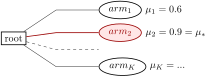
\includegraphics[scale=1.0]{onelevel-tree.pdf}\\
    \vspace{4em}
    a. search tree
  \end{minipage}
  \begin{minipage}[c]{0.5\linewidth}
    \centering
    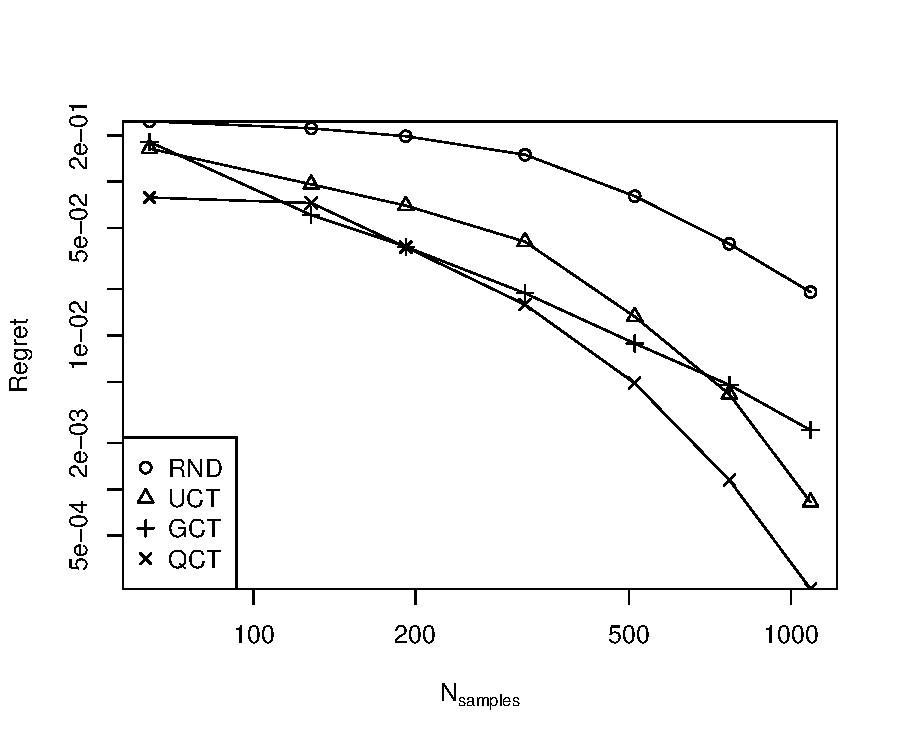
\includegraphics[scale=0.5]{flat-trilevel-k=64-uqb=8.pdf}\\
    b. regret vs. number of samples
  \end{minipage}
  \label{fig:mab-simple-regret}
  \caption{Simple regret in MAB}
\end{figure}

\subsection{Monte Carlo tree search}

\begin{figure}
  \begin{minipage}[c]{0.5\linewidth}
    \centering
    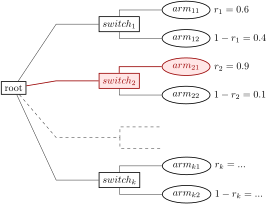
\includegraphics[scale=0.8]{twolevel-tree.pdf}\\
    a. search tree
  \end{minipage}
  \begin{minipage}[c]{0.5\linewidth}
    \centering
    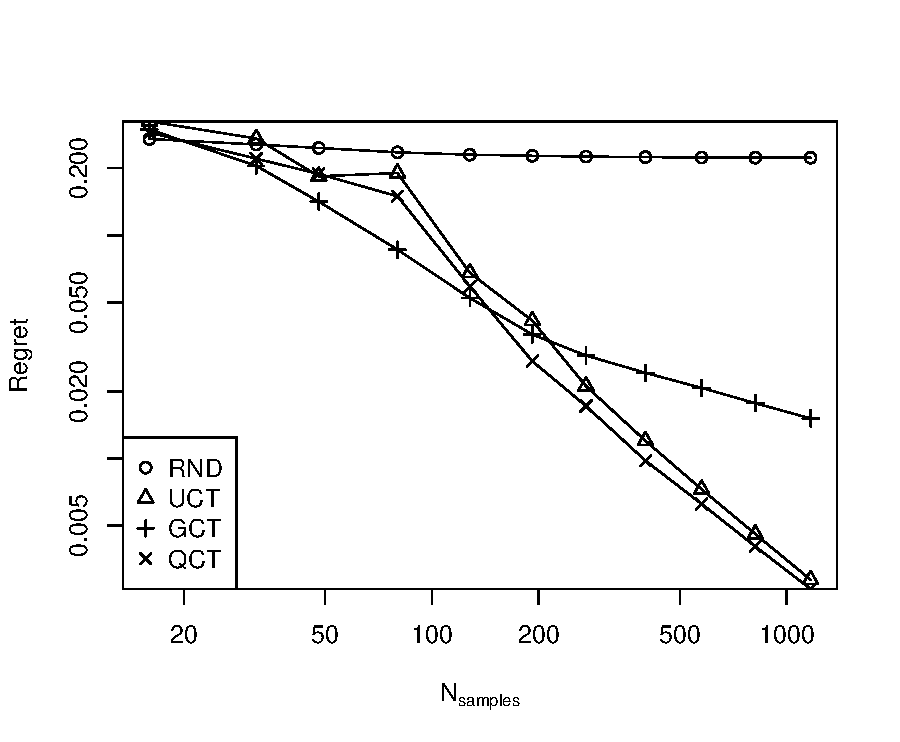
\includegraphics[scale=0.4]{tree-identity-k=16-uqb=8.pdf}\\ 
    b. 16 arms \\
    \vspace{1em}
    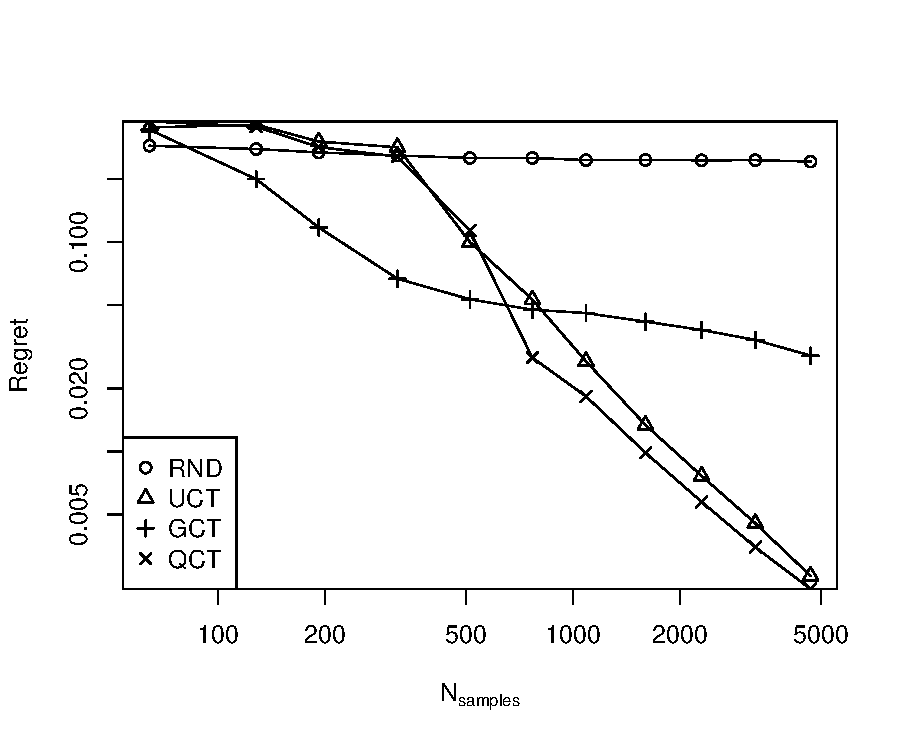
\includegraphics[scale=0.4]{tree-identity-k=64-uqb=8.pdf} \\
    c. 64 arms
 \end{minipage}
  \label{fig:mcts-regret}
  \caption{MCTS: a path to the best arm}
\end{figure}

\subsection{The sailing domain}


\begin{figure}[t]
  \begin{minipage}[b]{0.5\linewidth}
    \centering
    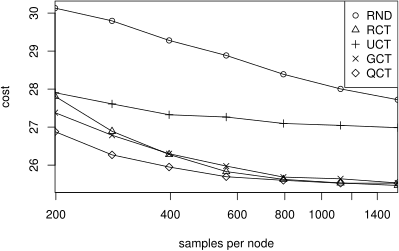
\includegraphics[scale=0.45]{costs-size=6-group=median.pdf}\\
    a. median cost
  \end{minipage}
  \begin{minipage}[b]{0.5\linewidth}
    \centering
    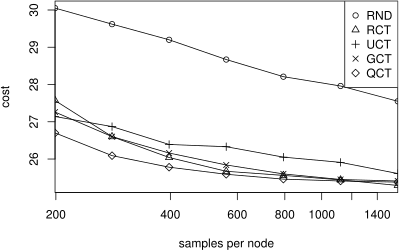
\includegraphics[scale=0.45]{costs-size=6-group=minimum.pdf}\\
    b. minimum cost
  \end{minipage}
  \caption{The sailing domain, $6\times 6$ lake, cost vs. number of playouts}
  \label{fig:sailing-cost-vs-nsamples}
\end{figure}

\begin{figure}[t]
  \begin{minipage}[b]{0.5\linewidth}
    \centering
    \includegraphics[scale=0.45]{costs-size=6-nsamples=199.pdf}\\
    a. 199 playouts\\
    \vspace{1em}
    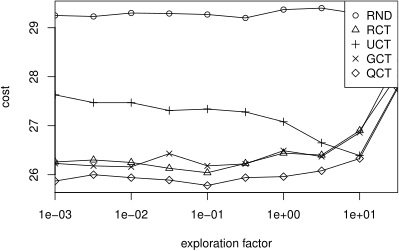
\includegraphics[scale=0.45]{costs-size=6-nsamples=397.pdf}\\
    b. 397 playouts\\
  \end{minipage}
  \begin{minipage}[b]{0.5\linewidth}
    \centering
    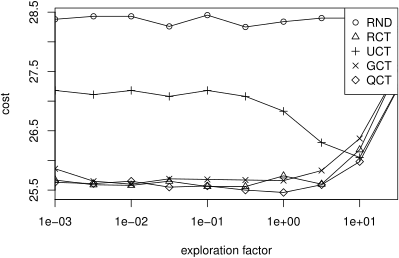
\includegraphics[scale=0.45]{costs-size=6-nsamples=793.pdf}\\
    c. 793 playouts\\
    \vspace{1em}
    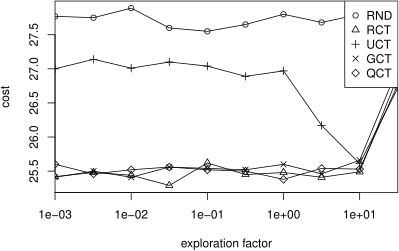
\includegraphics[scale=0.45]{costs-size=6-nsamples=1585.pdf}\\
    d. 1585 playouts\\
  \end{minipage}
  \caption{The sailing domain, $6\times 6$ lake, cost vs. factor}
  \label{fig:sailing-cost-vs-factor}
\end{figure}

\begin{figure}[t]
  \begin{minipage}[b]{0.333\linewidth}
    \centering
    \includegraphics[scale=0.35]{costs-size=3-nsamples=397.pdf}\\
    a. $3\times 3$ lake
  \end{minipage}
  \begin{minipage}[b]{0.333\linewidth}
    \centering
    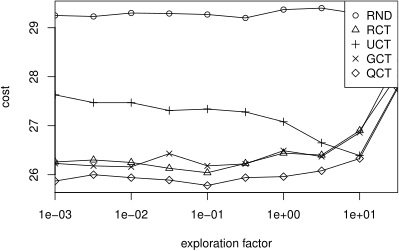
\includegraphics[scale=0.35]{costs-size=6-nsamples=397.pdf}\\
    b. $6\times 6$ lake
  \end{minipage}
  \begin{minipage}[b]{0.333\linewidth}
    \centering
    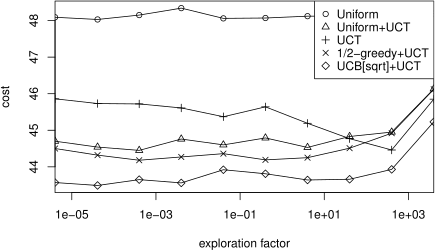
\includegraphics[scale=0.35]{costs-size=10-nsamples=397.pdf}\\
    b. $10\times 10$ lake
  \end{minipage}
  \caption{The sailing domain, 397 samples, cost vs. factor}
  \label{fig:sailing-lake-size}
\end{figure}

\begin{figure}[t]
  \begin{minipage}[b]{0.5\linewidth}
    \centering
    \includegraphics[scale=0.45]{rcq-size=6-nsamples=199.pdf}\\
    a. 199 playouts\\
    \vspace{1em}
    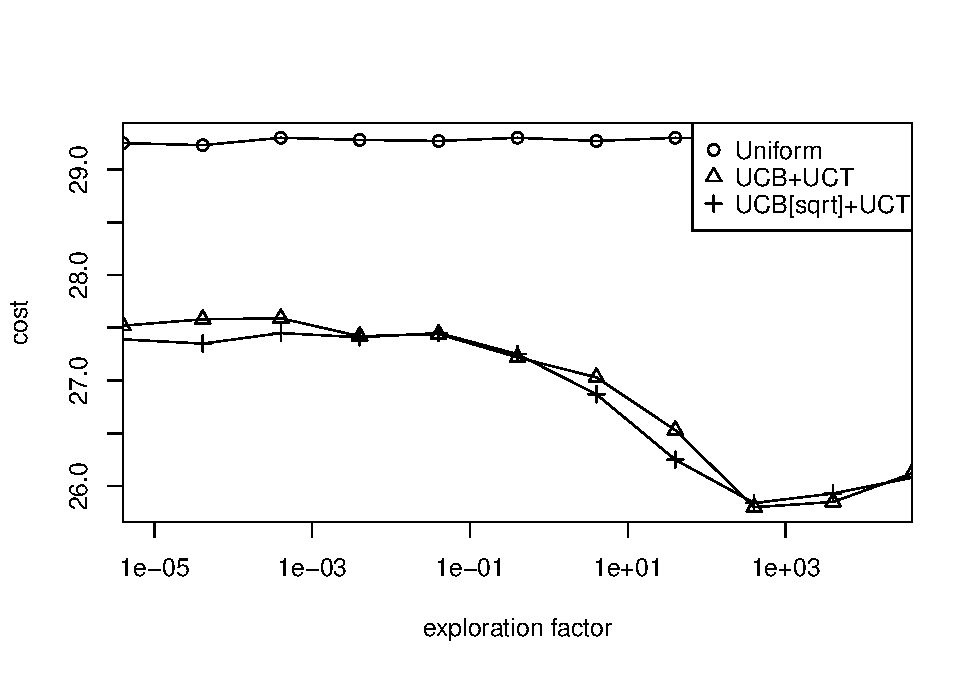
\includegraphics[scale=0.45]{rcq-size=6-nsamples=397.pdf}\\
    b. 397 playouts\\
  \end{minipage}
  \begin{minipage}[b]{0.5\linewidth}
    \centering
    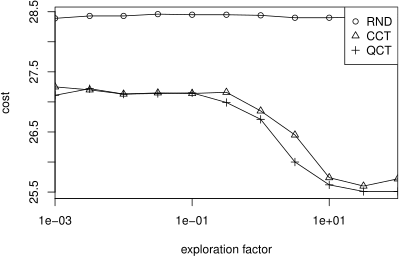
\includegraphics[scale=0.45]{rcq-size=6-nsamples=793.pdf}\\
    c. 793 playouts\\
    \vspace{1em}
    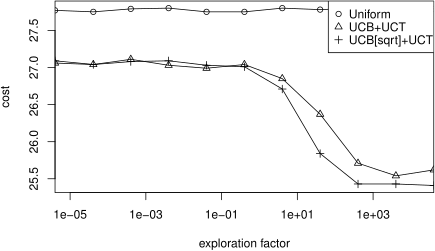
\includegraphics[scale=0.45]{rcq-size=6-nsamples=1585.pdf}\\
    d. 1585 playouts\\
  \end{minipage}
  \caption{The sailing domain, log vs. sqrt, $6\times 6$ lake}
  \label{fig:sailing-cost-vs-factor}
\end{figure}
%
%\begin{figure}[t]
%  \begin{minipage}[b]{0.5\linewidth} \centering
%    \includegraphics[scale=0.45,trim=0pt 0pt 0pt
%    0pt,clip]{sailing-size=13-factor=_5625.pdf}
%    {a. varying number of samples}
%  \end{minipage}
%  \begin{minipage}[b]{0.5\linewidth} \centering
%    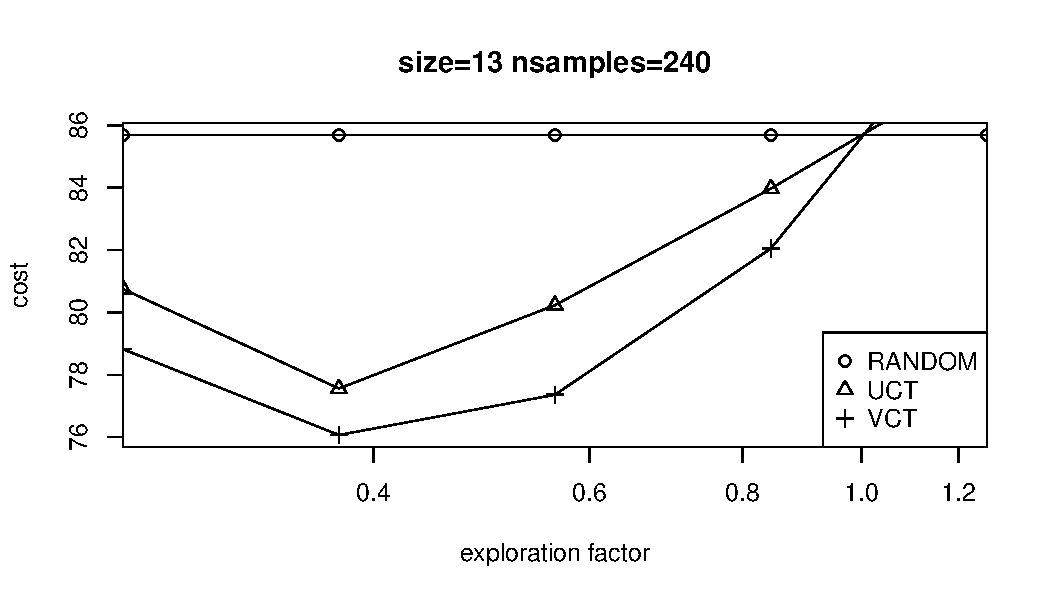
\includegraphics[scale=0.45,trim=0pt 0pt 0pt
%    0pt,clip]{sailing-size=13-nsamples=240.pdf}
%    {b. varying exploration factor}
%  \end{minipage}
%  \caption{The sailing domain, a larger lake}
%  \label{fig:sailing-13}
%\end{figure}

\section{Summary and Future Work}

\section*{Acknowledgments}

The research is partially supported by Israel
Science Foundation grant 305/09, by the Lynne and William Frankel
Center for Computer Sciences, and by the Paul Ivanier Center for
Robotics Research and Production Management.

\bibliographystyle{plain}
\bibliography{refs}

\pagebreak

\appendix

\section{Facts}

{\bf Chernoff bound (see \cite{Hagerup.chernoff}):} for $m$ independent random variables $X_1, X_2, ..., X_m$
taking values 0 or 1, $X=\sum_{i=1}^m X_i$, and $0\le\delta\le 1$:

\begin{equation}
\label{eq:chernoff-bound}
\Pr[X < (1-\delta)\IE[X]] < e^{-\delta^2\IE[X]/2}
\end{equation}

\section{Derivations}

\subsection{Finite-time regret bounds}

For an analysis of pure exploration of uniform and UCB algorithms, see also
\cite{Bubeck.pure}.


\subsubsection{$\varepsilon$-greedy}

For $0<\varepsilon\le1-\frac 1 K$ and $x_0>0$ (see Section 3, Proofs, in \cite{Auer.ucb}):

\begin{eqnarray}
\Pr(\overline X_j=\max_i\overline X_i)&\le&2\left(x_0\cdot \Pr\left\{T_j^R(n)\le x_0\right\} + \frac 2{\Delta_j^2}e^{-\Delta_j^2\lfloor x_0 \rfloor/2}\right)\nonumber\\
&\le&2\left(x_0\cdot \Pr\left\{T_j^R(n)\le x_0\right\} + \frac {2 \cdot
  e^{\Delta_j^2/2}}{\Delta_j^2}e^{-\Delta_j^2 x_0 /2}\right)
\end{eqnarray}

Number of times $\mu$ the $j$th arm is selected {\it randomly}:

\begin{equation}
\mu\triangleq\IE\left[T_j^R(n)\right]=\frac {n\varepsilon} K
\end{equation}

By choosing $x_0=\frac \mu 2$ and applying the Chernoff bound (\ref{eq:chernoff-bound}), obtain:

\begin{eqnarray}
\label{eq:pr-epsilon-greedy}
\Pr(\overline X_j=\max_i\overline X_i)&\le& 2\left(\frac {\mu}{2} e^{-\mu/8} + \frac {2e^{\Delta_j^2/2}}{\Delta_j^2}e^{-\Delta_j^2 \mu/4}\right)\nonumber\\
&\le&\left(\mu + \frac {4\sqrt e}{\Delta_j^2}\right)e^{-\Delta_j^2\mu/8}
\end{eqnarray}

A bound on the simple regret $r_\varepsilon$ of an
$\varepsilon$-greedy policy follows from substituting
(\ref{eq:pr-epsilon-greedy}) into (\ref{eq:simple-regret}):

\begin{eqnarray}
  \IE r_\varepsilon&\le&\sum_{j=1}^K\Delta_j\left(\mu + \frac {4\sqrt e}
{\Delta_j^2}\right)e^{-\Delta_j^2\mu/8}\nonumber\\
&\le&K\left(\mu + \frac {4\sqrt
    e}{\Delta_{\min}}\right)e^{-\Delta_{\min}^2\mu/8}
\label{eq:deriv-epsilon-greedy-b}
\end{eqnarray}

\subsubsection{UCB($\alpha$)}

$n_b$ pulls of the best arm and $n_j$ pulls of the $j$th arm are
achieved simultaneously when either 


\begin{equation}
\sqrt {\frac {\alpha \log n} {n_j-1}} \ge 1 + \sqrt { \frac {\alpha \log n} {n_b}}
\end{equation}

or

\begin{equation}
\sqrt {\frac {\alpha \log n} {n_j}} \le 1 + \sqrt { \frac {\alpha \log n} {n_b - 1}}
\label{eq:deriv-ucb-alpha-a}
\end{equation}

Inequality (\ref{eqn:deriv-ucb-alpha-a}) can be used to derive a lower
bound on the number of pulls of a non-optimal arm,  and, consequently, the upper
bound on the probability of selecting a non-optimal arm:

\begin{eqnarray}
\frac {\alpha \log n} {n_j}&\le& 1 + 2  \sqrt {\frac {\alpha \log n}
  {n_b-1}} + \frac {\alpha \log n} {n_b-1}\nonumber\\
n_j &\ge& \frac {\alpha \log n} {1+2 \sqrt {\frac {\alpha \log n}
    {n_b-1}} + \frac {\alpha \log n} {n_b-1}}\nonumber\\
    &\ge& \frac {\alpha \log n} {4} \mbox{ for } \alpha \log n \le n_b-1
\end{eqnarray}

The probability that the $j$th arm will be chosen can be bounded based
on the Chernoff inequality and the union bound:
\begin{equation}
P_j \le 2 \exp\left(-\frac {\alpha \Delta_j^2 \log n} 8 \right) = 2n^{\frac {-\alpha \Delta_j^2} 8}
\end{equation}

The expected simple regret of an UCB($\alpha$) algorithm is thus
bounded by the following inequality:
\begin{equation}
\IE r_{ucb} \le 2\sum_{j=1}^K \Delta_jn^{\frac {-\alpha \Delta_j^2} 8}
\label{eq:deriv-ucb-alpha-b}
\end{equation}

\cite{Bubeck.pure} provides for UCB($\alpha$) a similar bound,
polynomial in the number of pulls $n$.

\subsection{Asymptotic regret analysis}

Bounds (\ref{eq:deriv-epsilon-greedy-b}, \ref{eq:deriv-ucb-alpha-b}) where
derived ignoring dependency of the allocation on expected values
of non-optimal arms. Derivation of better bounds seems complicated; instead, insights
can be obtained by analysing  asymptotic behavior of each of the
algorithms in assumption that the sample mean approaches the expected
value. 

\subsubsection{$\varepsilon$-greedy}

\subsubsection{UCB($\alpha$)}

\end{document}
